\documentclass[%
 aip,
 apl,%
 amsmath,amssymb,
%preprint,%
 reprint,%
%author-year,%
%author-numerical,%
]{revtex4-1}

\usepackage{bm}% bold math
\usepackage{natbib}
\usepackage{graphicx}
\graphicspath{ {images/} }

% see http://tex.stackexchange.com/questions/153559/change-option-of-natbib-in-aip
%\renewcommand{\bibnumfmt}[1]{[#1] }

\begin{document}

%\preprint{AIP/123-QED}

\title[Micropatterned Substrates for Transport Measurements in Strained Graphene]{Micropatterned Substrates for Transport Measurements in Strained Graphene}

\author{J. Henry Hinnefeld}
 \affiliation{Department of Physics and Materials Research Laboratory, University of Illinois at Urbana-Champaign, 1110 West Green Street, Urbana, Illinois 61801, USA}
\author{Nadya Mason}
 \email{nadya@illinois.edu}
 \affiliation{Department of Physics and Materials Research Laboratory, University of Illinois at Urbana-Champaign, 1110 West Green Street, Urbana, Illinois 61801, USA}
 
\date{\today}

\begin{abstract}
Engineered substrates offer an interesting avenue towards graphene devices with tunable properties.
In particular, substrates which apply strain to graphene can expose unique behavior.
However, existing options for patterning strain-inducing substrates are not suitable for creating 
devices for electrical transport measurements.
In this letter we describe the fabrication of strain-inducing substrates suitable for transport measurements,
and we report both optical and transport measurements of graphene devices showing characteristics induced by these substrates.
\end{abstract}

%Use showkeys class option if keyword display desired
\keywords{graphene strain transport Raman}

\maketitle




%\section{Introduction / Motivation}
Graphene is a material with enormous potential for both scientific research and technical applications
\cite{novoselov2004electric,novoselov2005two,zhang2005experimental,geim2007rise}.
In particular, the ability to tune graphene's properties through the use of engineered substrates offers a practical
method to explore graphene's properties and modify them for specific applications\cite{guinea2010energy, zhou2007substrate}.
Engineered substrates offer a variety of avenues by which to modulate graphene's properties:
previous work has employed substrate topography\cite{Tomori2011},
electrostatic charge injection\cite{chiu2010controllable},
substrate lattice mis-match\cite{zhou2007substrate},
and ferroelectric polarization\cite{hinnefeld2016single}
to achieve a range of modifications to graphene's properties.

Of the various substrate engineering techniques, applying strain via substrate topography is particularly interesting
because of the large effect strain has on graphene's electrical 
properties\cite{guinea2010energy, pereira2009strain, levy2010strain}. 
To date however, the techniques used to produce strain in graphene are either not tunable\cite{levy2010strain}
or not amenable to performing electrical transport measurements on graphene
\cite{Tomori2011, mohiuddin2009uniaxial, ni2008uniaxial, gill2015mechanical}.
Here we demonstrate a fabrication procedure for producing engineered arrays of strain-generating features on standard silicon
substrates, and we report optical and transport measurements which display characteristics induced by these substrates.

%\section{Fabrication}

The process used to create the strain features on the substrate is illustrated schematically in Figures \ref{'fig:fab'}A-D.
First, an array of copper circles is deposited on a silicon chip having a 1 $\mu$m layer of thermal oxide using standard 
electron-beam lithography and evaporation techniques. The deposited copper is then used as a mask in a reactive ion etching 
(RIE) step to produce cylindrical pillars in the SiO$_2$ layer. For the devices described here the etch was performed in 
a PlasmaLab Freon RIE at 35 mtorr for 10 minutes 
using 100 W of incident power and 70 sccm of CF$_4$. After the etch, the copper mask is removed by immersing the chip 
in a 0.1M solution of ammonium persulfate for several hours. Finally, the chip is dipped in buffered oxide etchant 
(6:1 40\% NH$_4$F : 49\% HF) to sharpen the SiO$_2$ pillars produced during the RIE step into pointed, conical shapes. 
The BOE dip time is an important parameter which depends on the initial diameter of the pillars; for the the devices
described here BOE was found to etch the tip of the pillars at a constant rate of approximately 2 nm/s. 

\begin{figure}
\centering
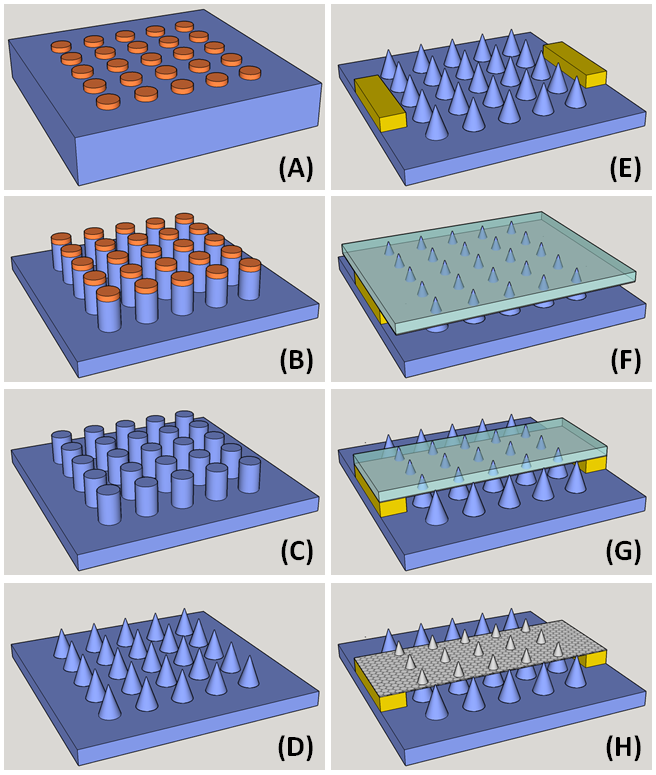
\includegraphics[width=\columnwidth]{Figure1}
\caption{Fabrication procedure for creating graphene devices on strain-array substrates.}
\label{'fig:fab'}
\end{figure}

\begin{figure}
\centering
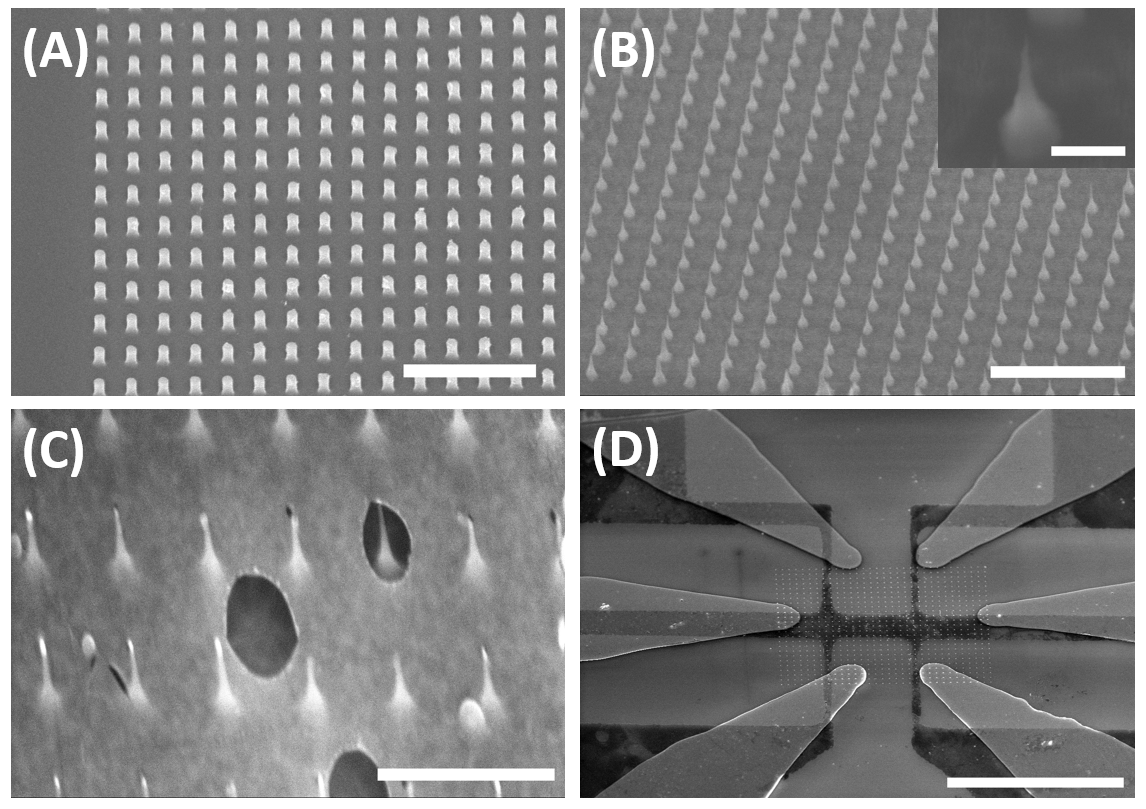
\includegraphics[width=\columnwidth]{Figure2}
\caption{SEM micrographs of substrates prepared by this method. 
(A) SiO$_2$ pillars before the BOE etch. The scale bar is 1$\mu$m.
(B) After the BOE dip the SiO$_2$ pillars are sharpened into cones with a tip diameter of less than 10 nm.
The scale bar is 1 $\mu$m. Inset: A single sharpened cone. The scale bar is 100 nm.
(C) For tight strain array spacings the graphene is suspended on the pointed tips of the substrate features.
Here the substrate is visible through rips in the graphene. The scale bar is 500 nm.
(D) After transfer the graphene is patterned in a Hall bar geometry. The six triangular features are Ti/Au
electrical leads. The scale bar is 20 $\mu$m.}
\label{'fig:sem'}
\end{figure}

Graphene devices are fabricated on substrates prepared by this method using the process shown in Figures \ref{'fig:fab'}E-F. 
First Ti/Au (5 nm/30 nm) leads and contact pads are defined and deposited using electron-beam lithography and evaporation. 
Next, a monolayer of graphene is grown using established chemical vapor deposition techniques\cite{Li2009}. 
The graphene is then transferred to the strain array substrate using standard polymer-assisted wet-transfer 
techniques\cite{li2009transfer}. The same polymer layer used to transfer the graphene is then used as a 
resist in an electron-beam lithography step. Next the exposed graphene is removed using a reactive ion etch 
(100 W, 50 mtorr, 20 sccm O$_2$, 30 s), yielding graphene in a Hall bar configuration. Finally the remaining 
polymer resist is dissolved in acetone and the chip is dried in a critical point drying apparatus. 
The critical point drying is necessary because for certain array spacings the graphene remains suspended between
strain features, and when the device is allowed to dry in air the surface tension 
of the evaporating solvent tears the suspended graphene.
Figure \ref{'fig:sem'} shows scanning electron microscope (SEM) micrographs of substrates and
graphene devices produced by this process.

%\section{Strain via Raman}

Optical measurements of graphene devices fabricated on substrates prepared by the process described above
confirm the presence of strain. Raman measurements are collected in a raster pattern across a 
20 $\mu$m  $\times$ 20 $\mu$m area (CHECK THIS). At each raster point the Raman G and 2D peak positions
are extracted; figures \ref{'fig:raman'}a and \ref{'fig:raman'}b summarize the extracted positions 
of the Raman G and 2D peaks, respectively, 
for graphene on strain array and flat substrates. 

For both the G and 2D peaks graphene on the patterned 
substrates displays a shifted peak position. Doping from charge impurities in the substrate is also known to 
shift Raman peak positions in graphene\cite{reina2008large, casiraghi2007raman}, however the ratio 
\begin{equation}
    r = \frac{\Delta \, \omega_{2D}}{\Delta \, \omega_{G}}
\end{equation}
(where $\Delta \, \omega_{G}$ is the shift in the Raman G peak position relative to its intrinsic value)
differs between the two mechanisms \cite{lee2012optical}. 
Experimental measurements \cite{zabel2012raman, metzger2009biaxial, ding2010stretchable} and theoretical \cite{mohr2010splitting, mohiuddin2009uniaxial} results place the ratio for strain between 2.25 and 2.8 and the ratio for doping at approximately 0.75 \cite{lee2012optical}. Figure \ref{'fig:raman'}c shows this ratio for each 
of the measured devices. For graphene on flat substrates $r$ remains near the 

\begin{figure}
\centering
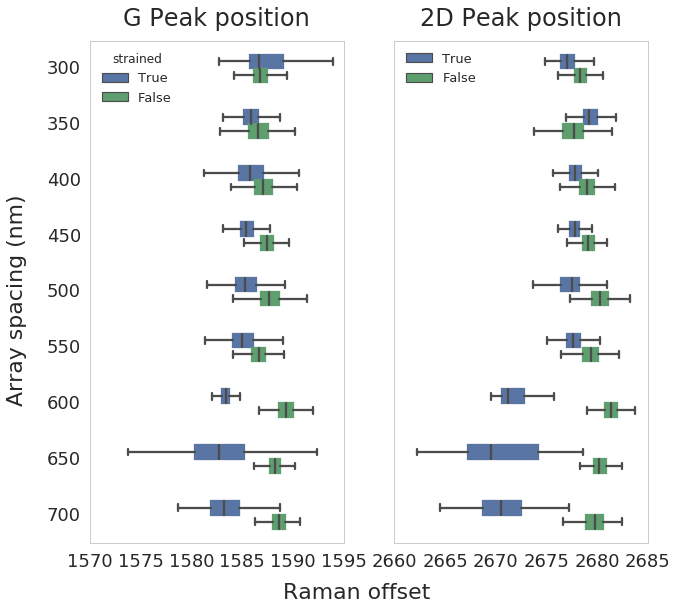
\includegraphics[width=\columnwidth]{Figure3}
\caption{Raman peak positions for graphene on micropatterned and flat substrates.}
\label{'fig:raman'}
\end{figure}

%\section{Transport - CB / localization}

Dirac point near XXX V, enhanced doping a function of the fabrication process as well as the thickness of the SiO$_2$ dielectric layer.

Figure \ref{'fig:transport'} shows the results of magneto-transport measurements performed on strain array and flat substrates.
Qualitative differences between the strained and unstrained devices are apparent: the control device displays a typical Landau level
fan pattern CITE SOMETHING, however the strain array device displays several resistance maxima not present in the control device.

We attribute these maxima to resonances induced by scattering from the strain array substrate. This analysis is corroborated by 
both the field and energy scales of the observed features: features persist up to field of approximately 1 T and extend over a
gate voltage range equivalent to approximately XXXX eV. Considering first the field dependence, we take the cyclotron radius
to be the relevant length scale.
\begin{equation}
    r_c = \frac{v_F m^*}{e B} = \frac{\hbar \sqrt{n \pi}}{e B}
\end{equation}
For a carrier density of $10^{11}$ cm$^{-2}$ and a field of 1 T corresponding the the field at which the transport features disappear, 
we find a cyclotron radius of 230 nm, in excellent agreement with the 250 nm spacing of the strain array features.

Next, we consider the energy dependence; here we approximate the system as a two-dimensional infinite well and calculate the length scale corresponding
to the observed energy scale.
\begin{equation}
\begin{split}
    E = \frac{\hbar^2 {k_F}^2}{2 m^* L^2} = \frac{m^* {v_F}^2}{2 L^2} = \frac{\hbar (n \pi)^{\frac{1}{2}} v_F}{2 L^2} \\
    \rightarrow L = \sqrt{\frac{\hbar (n \pi)^{\frac{1}{2}} v}{2 E}}
\end{split}
\end{equation}

\begin{figure*}
\centering
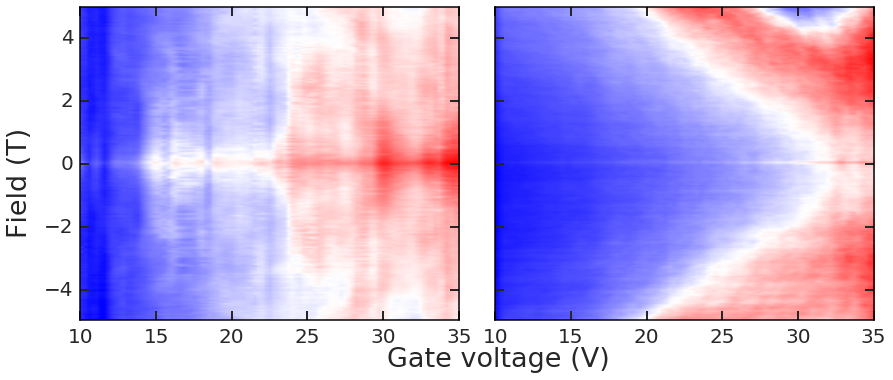
\includegraphics[width=1.5\columnwidth]{Figure4}
\caption{Device resistance as a function of gate voltage and field.}
\label{'fig:transport'}
\end{figure*}

\section*{REFERENCES}
\bibliographystyle{aipnum4-1}
\bibliography{strainarray}

\end{document}
%
% ****** End of file aipsamp.tex ******
